\section{Bluetooth BR/EDR (Basic Rate/Enhanced Data Rate)}
\subsection{Summary}
\begin{itemize}
	\item Applications: cable replacement, ad-hoc networking, WPAN 
	\item Standard: Industry standard of Bluetooth SIG (Special Interest Group): http://www.bluetooth.org 
	\begin{itemize}
		\item BT Spec V1.1:  Basis for 1. Basic-Rate-(BR-) products, $R_{max} = 0.7$ Mbps, IEEE 802.15.1-2002 
		\item BT Spec V1.2:  Adaptive FH  
		\item BT Spec V2.0:  Enhanced Data Rate (EDR), $R_{max}  = 2.1$ Mbps 
		\item BT Spec V2.1:  Secure Simple Pairing 
		\item BT Spec V3.0:  Alternative 802.11 MAC PHY (AMP), high speed (HS-) version, $\leq 24$ Mbps 
		\item BT Spec V4.0:  released 2010, BR/EDR and HS-option, and Bluetooth Low Energy 
	\end{itemize}
	\item Frequency Band: 2.4 GHz ISM-band, 79 channels with 1 MHz carrier spacing between 2402-2480 MHz
	\item Multiple Access
	\begin{itemize} 
		\item FHSS for interference mitigation (1600 hops/s, 625 us time slots, Time-Division-Duplexing) 
		\item FH-CDMA for piconet separation 
		\item Adaptive FH (AFH) to support coexistence with other systems, e.g. WLAN  
	\end{itemize}
	\item Modulation
	\begin{itemize}
		\item BR: GFSK, gross bit rate 1 Mbps  (Bluetooth symbol period is 1us)
		\item EDR: $\pi/4$-DQPSK or 8DPSK, gross bit rate 2 Mbps or 3 Mbps 
	\end{itemize}
	\item Error Control: CRC, FEC with $R=1/3$, $2/3$ or $R=1$ (no FEC), fast ARQ 
	\item Packet Length: 1-, 3- and 5-slot-packets (no FH during transmission), max. payload 1021 Bytes 
	\item Data Rates
	\begin{itemize}
		\item asynchronous:  $R \leq 531$ kbps (1-slot-packets only), $R \leq 1.3$ Mbps (symmetric), $R \leq 2.1$ Mbps (asymmetric) 
		\item synchronous:   $R = 64$ kbps (BR, voice), $R \leq 864$ kbps (EDR, high quality audio streaming) 
	\end{itemize}
	\item Power Classes:  class 1:  $P_{max} = 100$ mW (20 dBm), class 2:  $P_{max}  = 2.5$ mW (4 dBm), class 3:  $P_{max} = 1$ mW (0 dBm) 
	\item Sensitivity: specified -70 dBm, most devices achieve -80 dBm or better 
	\item Radio Range: indoor: 10 m with 1 mW power and 30 m with 100 mW 
	\item Architecture: 
	\begin{itemize}
		\item a Bluetooth-device can be master or slave 
		\item all Bluetooth-devices have a worldwide unique 48 bit Bluetooth Device Address (BD-Addr) 
		\item piconet:   1 master and up 7 slaves, synchronized to the master’s hopping sequence \\ 
		low power modes : park, hold or sniff state \\
		point-to-point and (asynchronous) broadcast communication 
		\item scatternet:  interconnected piconets (rarely used), a slave can participate in 2 piconets 
	\end{itemize}
	\item Protocol Stack: Core protocols like radio, baseband, etc. and Host Controller Interface (HCI) \\
	Profiles (e.g. Serial Port Profile, SPP) to provide interoperable services  
	and to adapt Bluetooth e.g. to audio-, TCP/IP- or AT-modem-applications 
	\item Security
	\begin{itemize}
		\item secure simple pairing based on public key protocols 
		\item challenge-response-authentication 
		\item stream ciperhing with 128 bit cipher key (SAFER+ algorithm) 
	\end{itemize}
	\item Some Disadvantages
	\begin{itemize}
		\item inquiry scan can last 5-10s 
		\item connecting time after pairing $\leq 30$ms
		\item current consumption and SW-stack too large for many low rate wireless devices/sensors \\
		\textit{typical current consumption of a bluetooth module with some profiles: 25 mA $@$3.0V for Tx (Peak $< 30$mA)}
		\item low cost for very high volumes only (some million chips / devices)  \\
		\textit{module solution with profiles costs 10-15 CHF $@$ 100k devices per year}
	\end{itemize}
\end{itemize}

\subsection{Piconet}
	\begin{tabular}{ll}
		\parbox{14cm}{
			A Bluetooth piconet is an ad-hoc network consisting of 1 master and 1 to 7 slaves 
			whereby all devices of the piconet have the same hopping sequence (and share the 
			same 1 MHz channel). The hopping sequence is derived from the master’s clock  
			and the master's Bluetooth device address BD-ADDR. 

			A number of independent piconets may exist in close proximity. Each piconet has a 
			different physical channel (that is a different master device and an independent timing 
			and hopping sequence.) 
			
			A Bluetooth device can never be a master of more than one piconet, since in BR/EDR the piconet
			is defined by synchronization to the master's Bluetooth clock. However, a Bluetooth device 
			may be a slave in many independent piconets. It does this on a time-division multiplexing basis.
			
			Two Bluetooth slaves can only communicate with each other via the Bluetooth master. The Bluetooth
			piconet is a star or point-to-multipoint network.
			
			When a master wants to connect to a slave with an unknown Bluetooth device address, then the piconet 
			connection procedure consists of
			\begin{enumerate}
				\item the inquiry procedure and
				\item the paging procedure.
			\end{enumerate}
			
			The connection procedure can last 5-10s.
		}	
		& \parbox{4cm}{
			\fbox{ 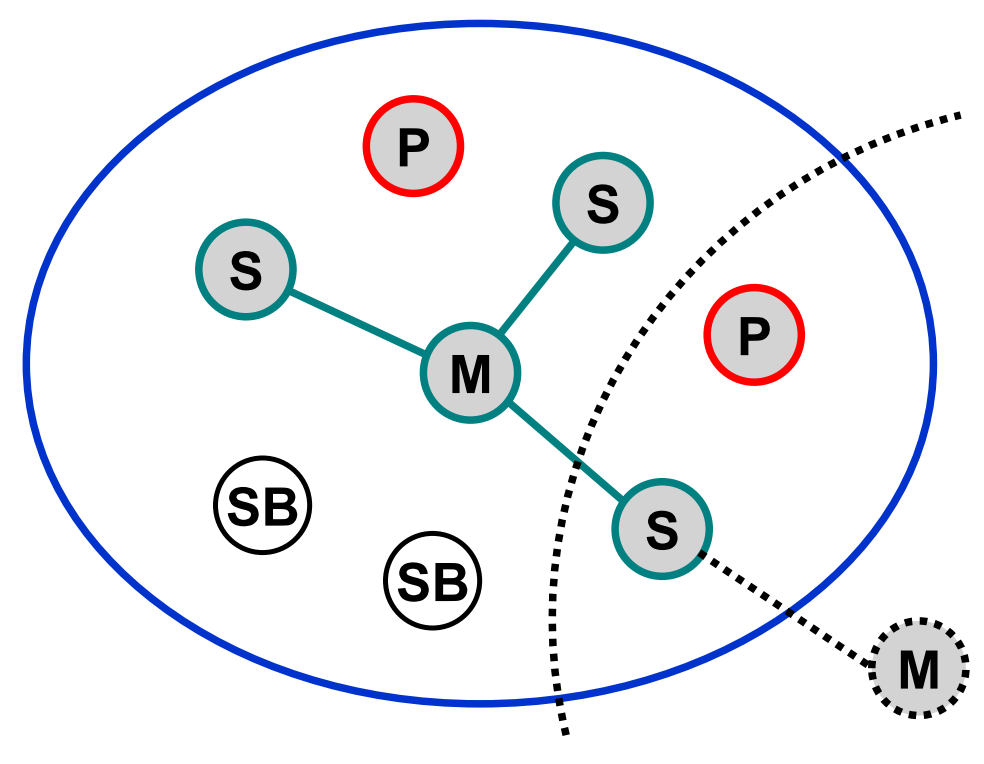
\includegraphics[width=4cm]{./bilder/bt-piconet.png}} \\ Piconet and Scatternet }
	\end{tabular}

\subsection{AFH - Adaptive Frequency Hopping}
	Adapted piconet physical channels can be used for connected devices that have AFH enabled. There are 
	two distinctions between basic and adapted piconet physical channels. The first is the same channel 
	mechanism that makes the slave frequency the same as the preceding master transmission. The second aspect 
	is that the adapted piconet physical channel may be based on less than the full 79 frequencies of the 
	basic piconet physical channel.
	
	AFH is used to improve resistance to radio frequency interference by avoiding the use of crowded frequencies
	(e.g. used by WLANs) in the hopping sequence.

\subsection{Packet transmission}
	In an EDR-packet there is a small guard time and synchronization sequence before payload. This is 
	a field used for physical layer change of modulation scheme (GFSK for the packet header and 4- or 8-PSK 
	for the payload). The packet header is GFSK-modulated in order that all Bluetooth devices can decode it.
	
	During the transmission of a multi-slot packet (e.g. 3 slots) the frequency f(k) of the master doesn't hop. When 
	the transmission is terminated, the frequency of the master hops to the next slot (e.g. f(k+3)). If there is a  
	collision in a slot during the transmission of a multi-slot packet, then the whole packet is destroyed. \\
	
	Bluetooth knows the following types of logical links:
	\begin{itemize}
		\item Synchronous Connection-Oriented \textbf{(SCO)} logical transport, point-to-point logical transport,  
		where there is no repetition of lost packets, but there are reserved slots at regular intervals 
		for maintaining the synchronous transport (e.g. for voice). 
		\item Extended Synchronous Connection-Oriented \textbf{(eSCO)} logical transport, where a repetition is possible 
		within a certain retransmission window right after the reserved slots.
		\item Asynchronous Connection-Oriented \textbf{(ACL)} logical transport, 
		\item Active Slave Broadcast \textbf{(ASB)} logical transport, used by master to communicate with active slaves
		\item Parked Slave Broadcast \textbf{(PSB)} logical transport, used by master to communicate with parked slaves
	\end{itemize}
	
	\begin{tabular}{ll}
		\parbox{9cm}{
			\fbox{ 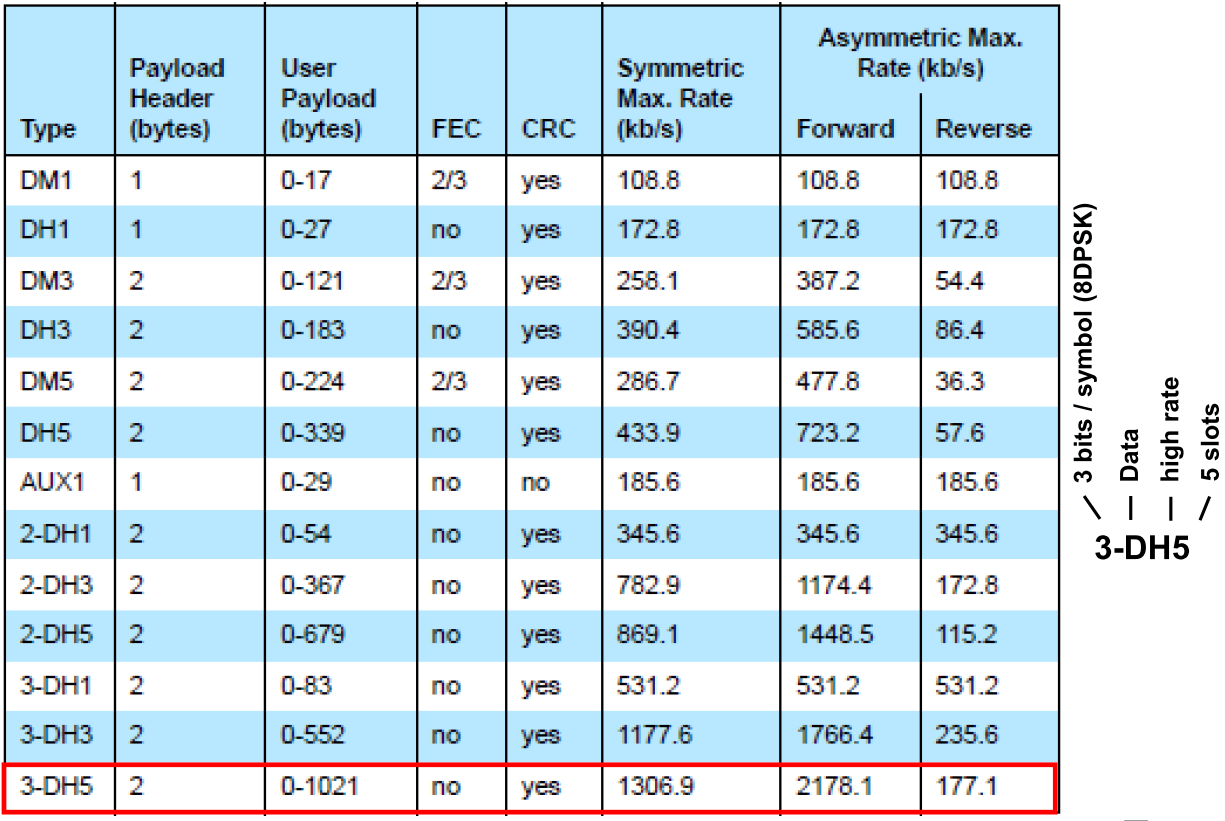
\includegraphics[width=8.5cm]{./bilder/bt-acl.png}} \\ ACL Packets 
		}	
		& \parbox{9cm}{
			\fbox{ 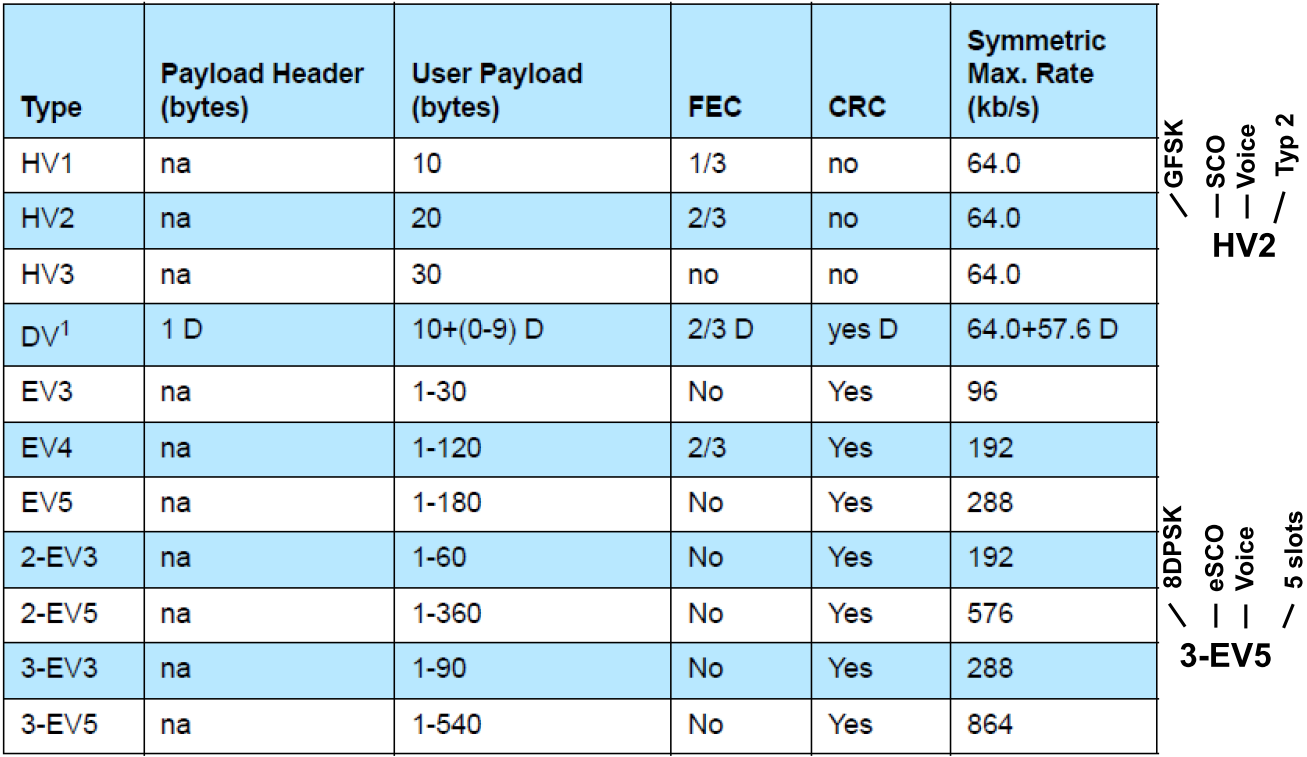
\includegraphics[width=8.5cm]{./bilder/bt-sco.png}} \\ Synchronous Packets 
		}
	\end{tabular}	\\

	The packets are transmitted in the first “part” of the time slots. The master sends always 
	in even slots. \\
	
	\begin{minipage}{16cm}
		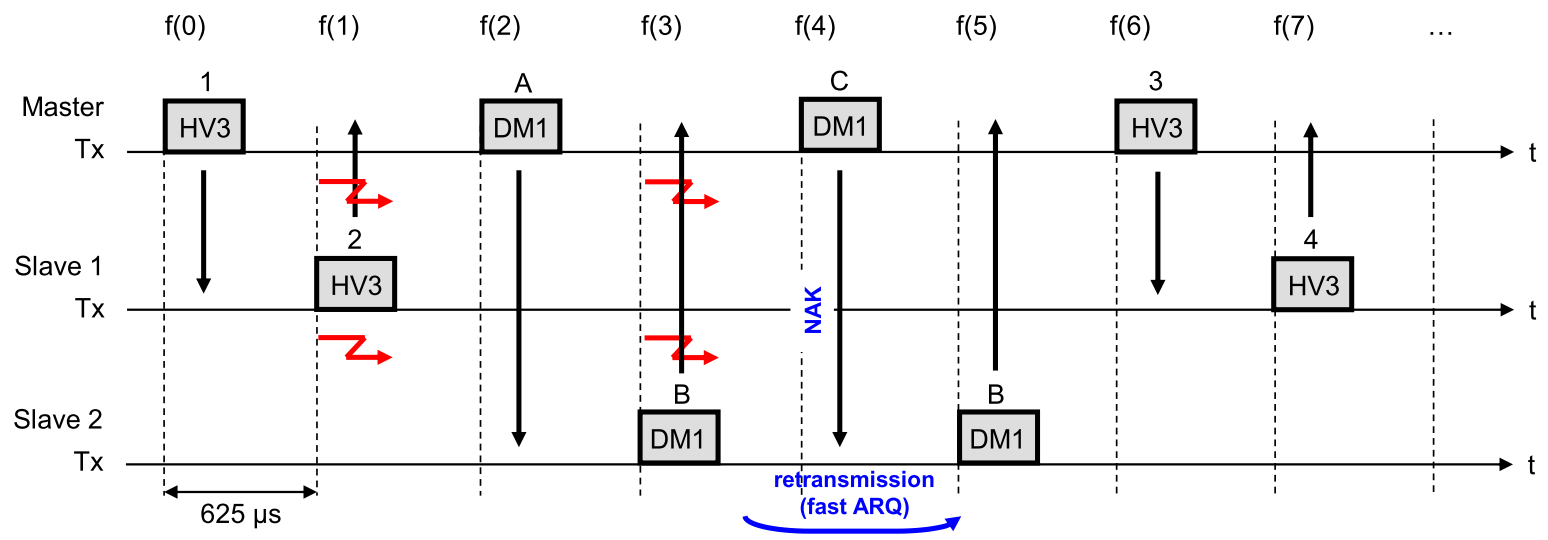
\includegraphics[width=16cm]{./bilder/bt-packet-transmission.png} 
	\end{minipage} \\
 

	HVx packets are periodically transmitted (e.g. in every 7th slot) to guaranty a time bounded 64 kb/s voice 
	service. HVx packets are not retransmitted (in contrast to the eSCO packets EVx 
	packets). 

	The slave has to retransmit the DM1-packet B because it receives a NAK in the header 
	of DM1-packet C. This procedure is also called fast Automatic Repeat reQuest ARQ. \\
	
	\textbf{Example:} Calculation of net data rate R for 3-DH1 (Up- or Downlink, with total 6 slots) \\
	$R = \frac{U_{pl}\cdot 8 \text{bit}}{N_{slots}\cdot T_{slot}} = \frac{83\cdot 8 \text{bit}}{6\cdot 625\mu s} = 177$kbps \\
	Where: $U_{pl}=$ User Payload [bytes], $N_{slots}=$ Total number of slots, $T_{slot}=625\mu$s = Slot time
	
	
	